114. \begin{figure}[ht!]
\center{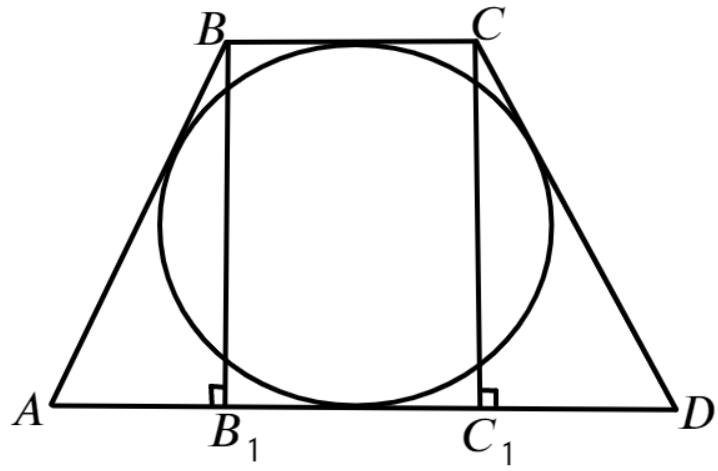
\includegraphics[scale=0.35]{g9-113.png}}
\end{figure}\\
Если трапеция описанная, суммы её противоположных сторон равны, поэтому\\ $AB=CD=\cfrac{49+16}{2}=\cfrac{65}{2}.$ Опустим высоты $BB_1$ и $CC_1,$ тогда $AB_1=C_1D=\cfrac{49-16}{2}=\cfrac{33}{2}$ и $BB_1=\sqrt{\cfrac{4225}{4}-\cfrac{1089}{4}}=28.$ Радиус вписанной окружности равен половине высоты, поэтому $R=28:2=14.$\\
